\section{Theory}
\subsection{Diffraction}
\paragraph{Principle of Huygens-Fresnel}
We will develop the theory of diffraction \cite{landau2} which will be usefull in the further progress
the theory. When start from geometrical optics, we notice that we use the approximation for the 
wavelength to be infinitely small. Taking into account the finite value of wavelength, we arrive at the
main concept of diffraction phenomena. Let's assume for an instance that the path of the light is limited by
opaque objects like an opening smaller than the beam of the light - then geometrical optics would predict 
total seperation between shadow and light after the opening. But with finite wavelengths, this seperation
is nullified by a complicated geometric intensity distribution fringing the areas of light,
depending on the shape and size of the opening. Clearly the smaller the openings are compared to the
wavelength this effects become stronger and stronger.
\begin{figure}[htpb]
    \centering
    \includegraphics[width=0.5\linewidth]{figures/beam}
    \caption{Sketch for the calculation of the intensity distribution Later. the Point $P$ denotes a distant
        point where we want to popagate the wave to, while $df$ at the surface of the aperture. For now 
        we assume the light incoming from the left side is parallel and monochromatic.}
    \label{fig:beam}
\end{figure}
\paragraph{Fraunhofer Diffraction}
We will not look at the non-dynamic case, leaving out all the factors $e^{-i\omega t}$ which can be appended
easily after if necessary. We start with a general wave incenting from the left side, with value $g(f)$ at the
surface of the aperture at a point $f$ (see figure \ref{fig:beam}). Then the wave at point $P$ due to the
outcoming wave of $f$ will
be proportional to $g(f)$, having lost
energy due to the enlarged surface proportional to $R$ and gaining a phase as well $e^{ikR}$ as well; 
the total wave at $P$ (which we denote with $\psi$) is thus the integral over the surface along d$f$: 
\begin{equation}
    \label{eq:int1}
    \psi_P \propto \int \frac{g(f) e^{ikR(f)}}{R(f)}\del f.
\end{equation}
The approximation is which can be sucessfull applied is fairly simply: For $P$ far enough away, the distance
$R$ is nearly the same for all points on the surface $f$, such that $R$ is not dependent on $f$ anymore and
we can pull it out of the integral
\begin{equation}
    \label{eq:int1}
    \psi_P \propto \int u(f) e^{ikR}\del f.
\end{equation}
The deeper point of this fairly easy assumption is that for distance $R \Rightarrow \infty$ the wavefunction
of an whatever shaped aperture is proportional to the Fourier Transform of the aperture. Lets assume
now a aperture function $g(x)$ of an one dimensional opening, then this translates into
\begin{equation}
    \psi_P \propto \mathcal{F} \left[g(k)\right ]_P
\end{equation}
where the dependency of $P$ in $g(x)$ comes from the factor $R$.
We have to think about fourier transformations before we can continue our studies.
\paragraph{Fourier Transformations}
We used the notation  $\mathcal{F} \left[g(k)\right ]_P$ which will be introduced here:
\begin{align}
f(x) &= \int_{-\infty}^{\infty} F(k)\exp(2\pi i kx)\del k\\
F(k) &= \mathcal{F}_x\left [f(x)\right ](k) =
\int_{-\infty}^{\infty} f(k)\exp(-2\pi i kx) \del x
\end{align}
The most important properties are:
\begin{align}
&\mathcal{F}\left [a f(x) + b g(x)\right ]
    = a F(k) + b G(k) 
    &\mbox{ (Linearity) }\\
&\mathcal{F}\left [f(x) * g(x)\right ](k)
    = \mathcal{F}\left [f(x)\right ]\mathcal{F}\left [g(x)\right ]
    \! &\mbox{ (Convolution) }\\
&\mathcal{F}_k\left [\left | F(k) \right |^2\right ](x)
   =  \int_{-\infty}^{\infty}\bar{f}(\tau)f(\tau + x) \del\tau 
   &\mbox{ (Wiener-Khinchin Theorem) }
\end{align}
Where in the last property $\bar{f}$ means the complex conjugation of $f$.
\paragraph{Intensity distributons}An important insight from electrodynamics is that the intensity density I of a
wave is proportional to the squared modulus of the complex wavefunction (We get the total intensity by
integrating over all points $P$).
Since this is enough for us to
know, we arrive at
\begin{equation}
    I_P \propto \psi_P^2 \propto \left ( \mathcal{F} \left[g(k)\right ]_P \right )^2 
\end{equation}
Now we can parametrize the Point $P$ in various scenarious. Let's assume a screen on the right side of
figure~\ref{fig:beam} at an angle $\theta$. Obviously the Distance $R$ can be parametrized such that
$R = x \sin \theta $, where $x$ is the horizontal distance (see figure~\ref{fig:beam2}).
\begin{figure}[htpb]
    \centering
    \includegraphics[width=0.5\linewidth]{figures/beam2}
    \caption{One dimensional parametrization of the aperture function.}
    \label{fig:beam2}
\end{figure}
Coming from this it is now possible to calculate the intensity from various one-dimensional aperture
functions
\begin{align}
    \label{eq:g1}
    g(x) = 
    \begin{cases}
        1 & \text{if } |x| \leq b/2 \\ 
        0 & \text{other }
    \end{cases} \\
    \Rightarrow \psi(\theta) \propto \int_{-b/2}^{b/2} \exp ^{-i k x \sin(\theta)} \del x
= \frac{2\sin ( k \frac{b}{2} \sin ( \theta )).
}{k \sin(\theta)} 
\end{align}
Such that we have for the Intensity density (dropping factor 4, see figure~\ref{fig:sinc1})
\begin{equation}
    \label{eq:sinc1}
    I(\theta) \propto \psi^2 \propto \frac{\sin^2 (k \frac{b}{2} \sin ( \theta )) }{k^2 \sin^2(\theta)} .
\end{equation}
\begin{figure}[htpb]
    \centering
    \includegraphics[width=0.8\linewidth]{figures/sinc1}
    \caption{This is the theoretic intensity distribution following equation~\eqref{eq:sinc1}. 
        We plugged in $\lambda = 632$nm and $b = 1 \mu$m. The density is normed to one.}
    \label{fig:sinc1}
\end{figure}

\subsection{Resolution of gratings}
\label{sec:resolution}

\subsection{Grating with $N$ lines}
\begin{equation}
    m \lambda = K \sin(\theta)
    \label{eq:N_lines_interference}
\end{equation}
